\section{Results}
\label{sec:results}

\begin{table*}[t]
\centering
\small
\setlength{\tabcolsep}{3.5pt}
\begin{tabular}{llll}
\toprule
Placement & Comparison (A $-$ B) & $\Delta\bar A$ [95\% CI] & $n$ \\
\midrule
1. PQK, steering metric & PQK $-$ cosine (baseline), R & $+0.06$ [$-0.07$, $+0.18$] & 3 \\
\midrule
\multirow{5}{*}{2. PQK, separation (QKSR)} & current $-$ previous-model features, R & $-0.02$ [$-0.06$, $+0.03$] & 3 \\
 & PQK $-$ RBF on the same angles, R & $+0.07$ [$-0.01$, $+0.15$] & 3 \\
 & PQK $-$ same circuit without CNOTs, R & $+0.04$ [$+0.04$, $+0.05$] & 3 \\
 & repaired (QKSR-v2) $-$ QKSR, R & $-0.07$ [$-0.11$, $-0.03$] & 3 \\
 & repaired PQK $-$ repaired RBF, R & $-0.04$ [$-0.08$, $+0.00$] & 3 \\
\midrule
\multirow{4}{*}{3. PQK, feature map} & PQK ridge $-$ linear head, A & $-17.33$ [$-19.07$, $-15.59$] & 3 \\
 & PQK without CNOTs $-$ linear head, A & $-10.40$ [$-11.10$, $-9.71$] & 3 \\
 & random Fourier features $-$ linear head, A & $-1.41$ [$-2.52$, $-0.31$] & 3 \\
 & random projection $-$ linear head, A & $-1.24$ [$-2.29$, $-0.19$] & 3 \\
\midrule
4. Holevo objective & von Neumann $\chi$ $-$ MCR$^2$ twin, R & $+0.06$ & 1 \\
5. Residual-POVM loss & POVM $-$ Gaussian twin, R & twin diverged (see text) & 1 \\
\midrule
\multirow{3}{*}{6. PGM, stand-alone} & PGM $-$ ridge, same statistics, R+A & $+0.09$ [$-0.23$, $+0.40$] & 11 \\
 & moment states $-$ per-sample states, R+A & $+0.07$ [$-0.02$, $+0.16$] & 11 \\
 & two-copy encoding $-$ amplitude encoding & $-3.6$ (R), $-6.5$ (A) & 5+5 \\
7. PGM, fused (SCF) & PGM source $-$ ridge source, 4 datasets & $-0.04$ [$-0.17$, $+0.08$] & 12 \\
\bottomrule
\end{tabular}
\caption{Every quantum placement against its classical twin. $\Delta\bar A$ in
points over paired runs; R: ImageNet-R, A: ImageNet-A. Rows 4--5 are one-run
screening results (no interval).}
\label{tab:quantum}
\end{table*}

\begin{table*}[t]
\centering
\small
\setlength{\tabcolsep}{2.2pt}
\resizebox{\textwidth}{!}{%
\begin{tabular}{lcccccccccc}
\toprule
& \multicolumn{2}{c}{CIFAR-100} & \multicolumn{2}{c}{ImageNet-R} & \multicolumn{2}{c}{ImageNet-A}
& \multicolumn{2}{c}{CUB-200} & \multicolumn{2}{c}{Average} \\
\cmidrule(lr){2-3}\cmidrule(lr){4-5}\cmidrule(lr){6-7}\cmidrule(lr){8-9}\cmidrule(lr){10-11}
Method & $\bar A$ & $A_B$ & $\bar A$ & $A_B$ & $\bar A$ & $A_B$ & $\bar A$ & $A_B$ & $\bar A$ & $A_B$ \\
\midrule
\multicolumn{11}{l}{\textit{Reported by \citet{rsiat} (exemplar-free, authors' partitions, one run)}} \\
L2P~\citep{l2p} & 89.23 & 84.29 & 75.46 & 69.77 & 49.39 & 41.71 & 67.05 & 56.25 & 70.28 & 63.01 \\
DualPrompt~\citep{dualprompt} & 87.36 & 82.30 & 73.10 & 67.18 & 53.71 & 41.67 & 77.47 & 66.54 & 72.91 & 64.42 \\
CODA-Prompt~\citep{codaprompt} & 91.30 & 86.85 & 77.97 & 72.27 & 53.54 & 42.73 & 84.00 & 73.37 & 76.70 & 68.80 \\
APER+Adapter~\citep{zhou2024aper} & 90.94 & 85.75 & 75.82 & 67.95 & 60.47 & 49.37 & 92.21 & 86.73 & 79.86 & 72.45 \\
EASE~\citep{ease} & 92.35 & 87.76 & 81.74 & 76.17 & 65.34 & 55.04 & 92.23 & 86.81 & 82.91 & 76.45 \\
SLCA~\citep{zhang2023slca} & 94.09 & 91.53 & 81.17 & 77.00 & 68.66 & 58.74 & 89.51 & 82.19 & 83.36 & 77.36 \\
RanPAC~\citep{mcdonnell2023ranpac} & 94.35 & 90.86 & 82.98 & 77.94 & 69.32 & 61.82 & 93.13 & 89.40 & 84.94 & 80.00 \\
MOS~\citep{mos} & 94.75 & 91.70 & 82.96 & 77.93 & 69.13 & 59.12 & 93.49 & 90.12 & 85.08 & 79.72 \\
SSIAT~\citep{ssiat} & 94.35 & 91.35 & 83.63 & 79.38 & 70.83 & 62.43 & 93.38 & 89.53 & 85.55 & 80.67 \\
RSIAT~\citep{rsiat} & 95.15 & 92.20 & 86.92 & 82.75 & 74.89 & 66.23 & 93.99 & 90.59 & 87.74 & 82.94 \\
\midrule
\multicolumn{11}{l}{\textit{Our runs (our partitions, mean $\pm$ SD over three seeds)}} \\
RSIAT (ours) & 95.02{\tiny$\pm$.21} & 92.03{\tiny$\pm$.19} & 87.11{\tiny$\pm$.49} & 82.55{\tiny$\pm$.05}
 & 74.26{\tiny$\pm$1.1} & 67.02{\tiny$\pm$1.1} & 93.53{\tiny$\pm$.79} & 88.47{\tiny$\pm$.31} & 87.48 & 82.52 \\
SCF, ridge (classical) & 95.22{\tiny$\pm$.20} & \textbf{92.41}{\tiny$\pm$.21} & 87.42{\tiny$\pm$.46} & 83.03{\tiny$\pm$.24}
 & \textbf{75.12}{\tiny$\pm$1.2} & \textbf{67.69}{\tiny$\pm$0.9} & \textbf{93.54}{\tiny$\pm$.88} & \textbf{88.85}{\tiny$\pm$.22} & \textbf{87.83} & \textbf{83.00} \\
SCF, PGM (quantum) & \textbf{95.23}{\tiny$\pm$.22} & 92.34{\tiny$\pm$.16} & \textbf{87.50}{\tiny$\pm$.43} & \textbf{83.07}{\tiny$\pm$.42}
 & 74.89{\tiny$\pm$1.0} & 67.65{\tiny$\pm$1.3} & 93.50{\tiny$\pm$.84} & 88.57{\tiny$\pm$.30} & 87.78 & 82.91 \\
\midrule
$\Delta$ ridge & $+$.20 {\tiny[.12,.28]} & $+$.38 {\tiny[.08,.69]} & $+$.32 {\tiny[.12,.51]} & $+$.48 {\tiny[.02,.94]}
 & $+$.85 {\tiny[.62,1.08]} & $+$.67 {\tiny[$-$.20,1.54]} & $+$.02 {\tiny[$-$.24,.27]} & $+$.38 {\tiny[.16,.61]} & $+$.35 & $+$.48 \\
$\Delta$ PGM & $+$.22 {\tiny[.15,.28]} & $+$.31 {\tiny[.18,.43]} & $+$.39 {\tiny[.25,.53]} & $+$.52 {\tiny[$-$.41,1.45]}
 & $+$.63 {\tiny[$-$.10,1.36]} & $+$.62 {\tiny[$-$.08,1.32]} & $-$.03 {\tiny[$-$.18,.12]} & $+$.10 {\tiny[.05,.16]} & $+$.30 & $+$.39 \\
\bottomrule
\end{tabular}}
\caption{Exemplar-free CIL with ViT-B/16-IN21K on four benchmarks. Top: results
reported in Table~1 of \citet{rsiat} on the authors' partitions (one run each);
they are not directly comparable with ours. Bottom: our runs, mean $\pm$ SD over
seeds 1993, 2015 and 2026; $\Delta$: paired difference of score fusion to RSIAT
in the same runs, with 95\% CI. Fusion weights were frozen on the tuning group
(ridge $w=0.25$, PGM $w=0.5$). Bold: best of our runs.}
\label{tab:main}
\end{table*}

\paragraph{No quantum component credibly beats its twin.}
Table~\ref{tab:quantum} is the main result of this study. Of the comparisons
with intervals, all but one contain zero or lie below it. The exception, the
separation kernel against the same circuit without CNOTs, is $+0.04$ points of
$\bar A$; the PQK also keeps old tasks better than the RBF twin (final accuracy
$+0.22$, $[+0.05,+0.39]$), but its gain in $\bar A$ is not resolved. The PQK as
a feature map and the richer two-copy encoding are clearly harmful. The PGM
matches ridge regression on the same statistics, alone and fused, as the
least-squares equivalence and Propositions~\ref{prop:unitary}--\ref{prop:shrink}
predict. The two training-time density-matrix objectives were stopped at
screening: the Holevo objective did not change final accuracy ($-0.18$ against
the four-run baseline mean, pre-registered threshold $+0.5$) and its classical
twin did as well. The Gaussian twin of the POVM loss diverged in task~1,
because its saturated softmax produced a near-zero gradient during the
calibration of $\lambda$, which then hit its upper bound; that comparison is
therefore not valid.

\paragraph{Repairing the separation kernel does not help.}
Against the baseline in the same environment, QKSR changes $\bar A$ by $+0.05$
($[-0.18,+0.28]$, $n=3$) while reducing forgetting by $0.54$
($[0.38,0.69]$). Its repaired version, which removes the weaknesses found by
the probe (Section~\ref{sec:qksr-analysis}), is worse than QKSR by $0.07$
points, and with the repair the PQK and its RBF twin become indistinguishable.

\paragraph{A classical fusion helps.}
Table~\ref{tab:main} gives the fusion results, which do not depend on the
quantum source. Final accuracy rises on all four datasets, by $+0.38$ to
$+0.67$ with the ridge source, and the interval excludes zero on three.
Average accuracy rises on CIFAR-100, ImageNet-R and ImageNet-A but not on
CUB-200, where the gain appears only in the last 3 of 20 stages; the
pre-registered transfer test to the two held-out datasets therefore failed
(Appendix~\ref{app:tests}). The ridge and PGM sources track each other at every
stage (Figure~\ref{fig:stage}, Appendix~\ref{app:figures}).

\paragraph{Position among published methods.}
Table~\ref{tab:main} and Figure~\ref{fig:comparison} place our runs next to
nine exemplar-free methods with the same backbone and task splits, as reported
by \citet{rsiat}. These numbers come from other partitions and single runs, so
they locate our results but do not test them; on the authors' partitions our
code reproduces the published RSIAT row to within $0.01$. With this caveat,
fusion's final accuracy is above every reported method on CIFAR-100,
ImageNet-R and ImageNet-A, and below the four strongest on CUB-200, where our
baseline is itself $2.1$ points below the published one. Exemplar-based methods
are compared in Appendix~\ref{app:exemplar}.

\begin{figure*}[t]
\centering
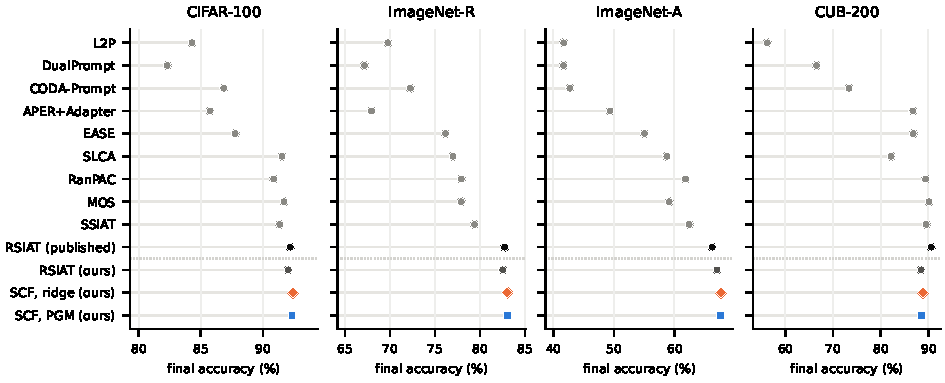
\includegraphics[width=\textwidth]{figures/comparison.pdf}
\caption{Final accuracy of nine exemplar-free methods (grey) and RSIAT (black) as reported by \citet{rsiat}, and of our runs (below the dotted line; mean over three seeds, our partitions). Orange: fusion with the classical ridge score; blue: with the quantum PGM score. Published and our numbers use different partitions.}
\label{fig:comparison}
\end{figure*}
